\documentclass[12pt]{scrartcl}
\input{../styles/Packages.tex}
\input{../styles/FormatAndHeader.tex}
\usepackage{tikz}

\usetikzlibrary{positioning}
\tikzset{
node of list/.style = { 
             draw, 
             fill=orange!20, 
             minimum height=6mm, 
             minimum width=6mm,
             node distance=6mm
   },
link/.style = {
     -stealth,
     shorten >=1pt
     },
array element/.style = {
    draw, fill=white,
    minimum width = 6mm,
    minimum height = 10mm
  }
}

\def\LinkedList#1{%
  \foreach \element in \list {
     \node[node of list, right = of aux, name=ele] {\element};
     \draw[link] (aux) -- (ele);
     \coordinate (aux) at (ele.east);
  } 
}
\usepackage{graphicx}

\setcounter{sheetnr}{6} % Nummer des Übungsblattes
\setcounter{exnum}{1} % Nummer der Aufgabe

% Beginn des eigentlichen Dokuments

\begin{document}

% Aufgabe 1
\exercise{Graphenrepräsentation}
\begin{enumerate}
  \item $G_2$ ist gerichtet. \\
  Begründung: Wenn der Graph ungerichtet wäre, gibt es für eine Kante $(i, j)$ in dem Graph immer eine gegenseitige Kante $(j,i)$. Aber z.B. für 
  die Kante (2,6), gibt es in $G_2$ keine Kante (6,2).\\
  Keine Ahnung, ob $G_2$ gewichtet ist. \\
  Begründung: Da in der Kanteliste keine Gewichtinformation erhalten ist.

  \item Graph $G_1$\\
  \begin{tikzpicture}[node distance={35mm}, thick, main/.style = {draw, circle}] 
    \node[main] (1) {$1$}; 
    \node[main] (3) [right of=1] {$3$}; 
    \node[main] (5) [right of=3] {$5$}; 
    \node[main] (4) [above of=3] {$4$}; 
    \node[main] (2) [below of=5] {$2$}; 
    \node[main] (6) [below right of=5] {$6$};
    \draw[->] (1) -- node[midway, below, pos=0.5] {5} (3) ; 
    \draw[->] (2) -- node[midway, below, sloped, pos=0.5] {8} (6) ; 
    \draw[->] (3) -- node[midway, below, sloped, pos=0.5] {6} (5) ; 
    \draw[->] (4) -- node[midway, below, sloped, pos=0.5] {9} (1) ; 
    \draw[->] (4) -- node[midway, below, sloped, pos=0.5] {1} (5) ; 
    \draw[->] (5) -- node[midway, below, sloped, pos=0.5] {2} (2) ; 
    \draw[->] (6) -- node[midway, below, sloped, pos=0.5] {2} (5) ;
    \end{tikzpicture} 

    \item Adjazenzliste, wobei der erste Element die Zielkonten ist und der zweite Element der Gewicht der Kante ist.\\
    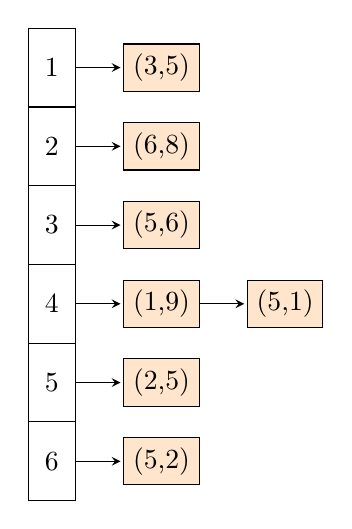
\begin{tikzpicture}
        \foreach \index/\list in {1/{(3,5)}, 2/{(6,8)}, 3/{(5,6)}, 4/{(1,9),(5,1)}, 5/{(2,5)}, 6/{(5,2)}} {
           \node[array element] (aux) at (0,-\index) {\index};
           \LinkedList{\list}
        }   
    \end{tikzpicture}

    \item Adjazenzmatrix\\
    \begin{tikzpicture}

        \matrix[matrix of math nodes,left delimiter = (,right delimiter = ),row sep=10pt,column sep = 10pt] (m) {
        0&0&1&1&0&0\\    0&0&0&0&1&1\\    1&0&0&0&1&0\\ 1&0&0&0&1&0\\ 0&1&1&1&0&1\\ 0&1&0&0&1&0\\   };
        
        \draw (m-1-2.north west) -- (m-1-2.south west)-- (m-5-6.south west) -- (m-5-6.south east) -- (m-5-6.north east) -- (m-1-6.north east) -- cycle;
        %the previous line can be replaced by \draw (m-1-1.north west) rectangle (m-2-2.south east);
    \end{tikzpicture}
    \\Da die Matrix symmetrisch ist, kann der markierte Teil entfernt werden.

    \item Knotenliste\\
    $G_2$ = \{6, 12, \underline{2,2,3}, \underline{3,1,5,6}, \underline{2,1,6}, \underline{3,4,5,6}, \underline{1,2}, \underline{1,3}\}

\end{enumerate}

\exercise{Breitensuche}
\begin{enumerate}
    \item Startknoten $C$: C,A,G,B,D,E,F
    \item Startknoten $F$: F,E,G,D,C,A,B
\end{enumerate}

\exercise{Präfix-Baum}
    \begin{enumerate}
        \item Präfix-Baum
        \begin{figure}[!h]
            \centering
              \includegraphics[width=0.5\textwidth]{Patrix.png}
            \caption{Präfix-Baum}
          \end{figure}
        \item Patricia-Baum
        \begin{figure}[!h]
            \centering
              \includegraphics[width=0.5\textwidth]{Patricia.png}
            \caption{Patricia-Baum}
          \end{figure}
    \end{enumerate}
    

\end{document}
